\documentclass{article}
\usepackage[utf8]{inputenc}
\usepackage{mathptmx}
\usepackage{microtype}

\usepackage{graphicx}
\graphicspath{{images/}}
\usepackage{subcaption}
\usepackage{float}
\usepackage{amsmath}

\usepackage{listings}
\lstdefinestyle{withframe}{frame=single}
\lstset{style=withframe}

\title{CS5234 Project Report}

\author{
  Chan Wai Hap (Axxxxxx) \\
  \texttt{xxxxx@u.nus.edu}
  \and
  Lu Wei (A0040955E) \\
  \texttt{wei.lu@u.nus.edu}
}

\begin{document}

\maketitle

\tableofcontents

\pagebreak

\section{Overview}
The density of a graph is defined as the number of edges divided by the number of nodes.

\begin{equation}
  \rho(G) = \frac{m}{n}
\end{equation}

Where $m$ is the number of edges and $n$ is the number of nodes of graph $G$. This is a convention we are going to use consistently for the rest of this report.

A dense subgraph is induced by a set of nodes in the original graph with many edges connecting them. The problem of finding the densest subgraph for undirected graphs is first formalized by A. V. Goldberg in 1984 (REFERENCE). He proposed a polynomial time exact algorithm for both unweighted and weighted graphs. It has been an active area research since. This class of problems are interesting not just from a theoretical perspective, they also have a lot of practical applications, such as community detection in social networks, web link spam detection for search engines, and correlation mining for gene, item or time series datasets. Such graph datasets are usually large with millions and even billions of nodes, which makes poly-time algorithm impractical. This prompts research in the direction of both distributed and approximation algorithms.

In our project, we limit the scope of our investigation to unweighted and undirect graphs. First, we explored both exact and approximation algorithms from existing literature for the densest subgraph problem, and formulated a distributed exact algorithm. For experimentation, we implemented Goldberg's exact algorithm, which we used to produce baselines for various datasets we experimented with. We then replicated and improved a MapReduce implementation of an approximation algorithm by Bahman et al in Hadoop – a distributed big data processing framework built on top of the MapReduce computational model. Last but not least, we also adopted the same approximation algorithm to a distributed graph processing framework named Giraph. We will present challenges and key lessons learned and compare the Hadoop and Giraph implementations.

\section{Algorithms and Theory}
In this section, we will introduce Goldberg's exact algorithm and briefly cover several approximation algorithms. Lastly, we will present our distributed exact algorithms and two possible realizations.

\subsection{Exact Algorithm}
The key idea of Goldberg's exact algorithm is to convert the original undirected, unweighted graph into a flow network as illustrated below:

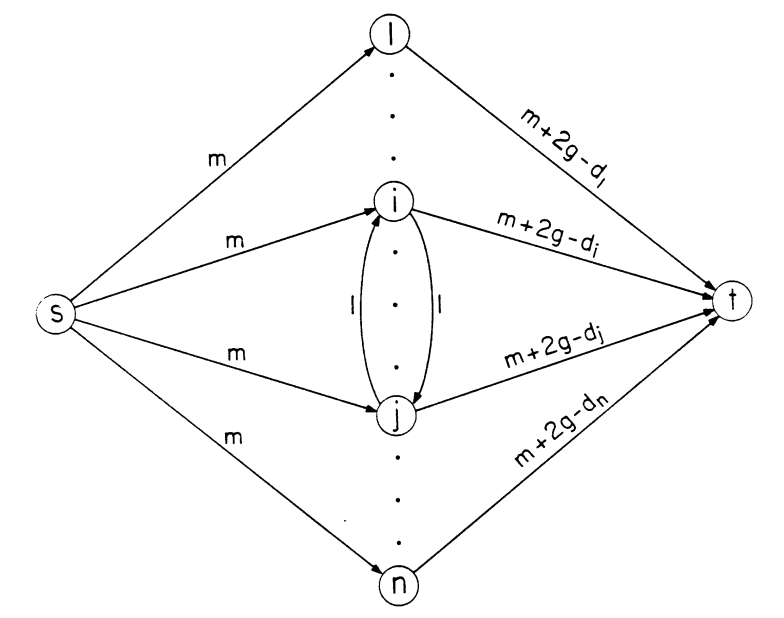
\includegraphics[width=\columnwidth]{goldberg_network.png}

Comparing to the original graph with nodes $V$ and edges $E$, the network has two nodes added: the source $s$ and the sink $t$: $V_N = V + \{s, t\}$, and $m + 2n$ edges added: $|E_N| = 2|E| + 2|N| = 2m + 2n$. Every original unweight and undirected edge is converted to two directed edges each with capacity 1. The capacity from $s$ to every node in the original graph is $m$; and the capacity from every node $i$ in the original graph to $t$ is assigned $m + 2g - d_i$, where $d_i$ is the degree of node $i$ in the original graph, and $g$ is a guessed value which the algorithm is going to iteratively ``sandwich'' by finding the min-cut until $g$ converges to the density of the densest subgraph.

The pseudocode for the algorithm is as below:

\begin{lstlisting}[mathescape=true]
  l=0, u=m, $V_1 = \emptyset$
  while $u - l > \frac{1}{n(n-1)}$ do
    $g = \frac{u+l}{2}$
    Construct network the updated g: $N = (V_N, E_N, g)$
    Find min-cut (S, T)
    if S = \{s\}
      u = g
    else
      l = g
      $V_1 = S - {s}$
  end
\end{lstlisting}

The intuition here is that the min-cut either goes throught all the out-edges of source node $s$, which looks like Case 1 below, or it doesn't (Case 2). In Case 1, the min-cut $c(S, T) = mn$; while for Case 2, the min-cut $c(S, T) = mn + 2n_1(g - \rho_1)$, where $n_1$ is the number of nodes in the subgraph induced by $V_1$ and $\rho_1$ is the density of the same subgraph. For detailed derivation please refer to the original paper (REFERENCE). Notice that the $mn$ term appears in both cases, so for Case 2 to be the min-cut, it has to be the case that $2n_1(g - \rho_1) < 0 \Rightarrow g < \rho_1 \leq \rho^*$ where $\rho^*$ is the densest subgraph density. It follows that when Case 1 is the min-cut, $g > \rho^*$.

\begin{figure}[H]
  \centering
  \begin{subfigure}{.48\textwidth}
    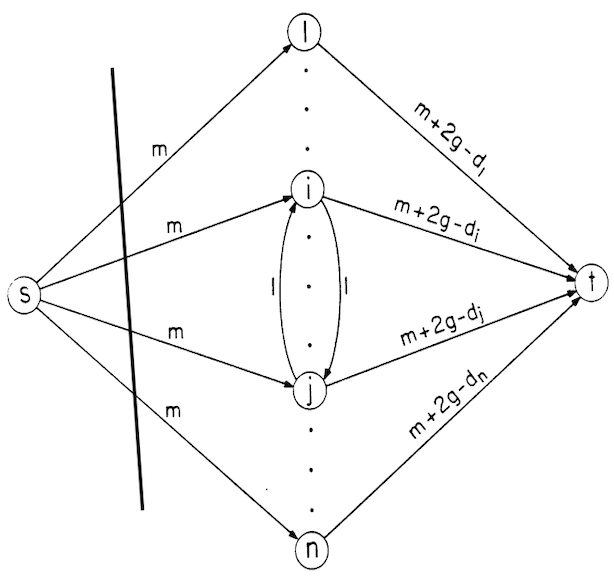
\includegraphics[width=\textwidth]{goldberg_network_cut1.png}
    \caption{Case 1}
  \end{subfigure}
  \begin{subfigure}{.48\textwidth}
    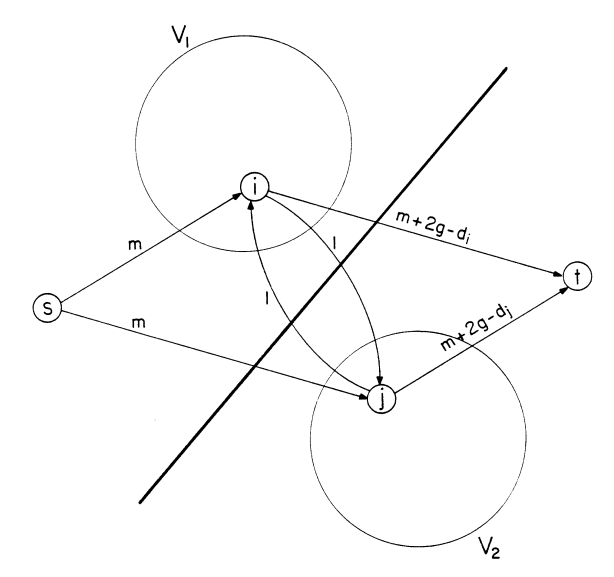
\includegraphics[width=\textwidth]{goldberg_network_cut2.png}
    \caption{Case 2}
  \end{subfigure}
\end{figure}

Since the value of $g$ is determined through binary search in the range of $[\frac{1}{n(n-1)}, m]$, it requires $log(n(n-1) \cdot m) = O(log(n^4)) = O(logn)$ iterations to terminate. Each iteration's running time is bounded by the time spent finding the min-cut in the contructed flow network.

There's extensive literature on finding s-t min-cut. The best known exact algorithm for general graphs is by Nagamochi and Ibaraki, which runs in time $O(mn + n^2logn)$ (REFERENCE). In comparison, the classic push-relabel algorithm by Goldberg and Tarjan (REFERENCE) runs in $O(n^3)$ time for a sequential implementation. Therefore for very dense subgraphs $m \approx n^2$, the best known min-cut algorithm's time complexity is also bounded by $O(n^3)$. Using $O(n^3)$ as the upper bound, the Goldberg densest subgraph algorithm described above has running time of $O(n^3logn)$.

We apprciate the cleverness of this algorithm in which one graph problem (densest subgraph) is translated to another graph problem (min-cut) through converting the original graph to a network flow with carefully assigned capacities. This is a common and effective technique we have come across while conducting literature review for this project.

\subsection{Approximation Algorithms}
We would like to focus on one approximation algorithm for finding densest subgraph in this section. It is proposed by Bahmani, Kumar, and Vassilvitskii (REFERENCE). The algorithm provides a $2 + 2\varepsilon$ approximation solution that completes in $O((m+n)logn$ time for a sequential implementation. We find this algorithm most impressive among its kind for the following reasons:

\begin{enumerate}
  \item Its distributed implementation completes in $O(logn)$ rounds,
  \item The algorithm itself is extremely simple, and
  \item It provides great close-to-truth approximation on real-world data.
\end{enumerate}

The key idea of this algorithm is to repeatedly remove small-degree nodes until the graph is empty. The intermediate subgraph with the highest density is the approximate solution to the densest subgraph problem. Below is the pseudocode:

\begin{lstlisting}[mathescape=true]
  $V_S, \tilde{V} = V$
  while $V_S \neq \emptyset$ do
    $V_R = \{i \in V_S | deg_S(i) \leq 2(1+\varepsilon)\rho_S\}$
    $V_S = V_S \ V_R$
    if $\tilde{\rho} < \rho_S$
      $\tilde{V} = V_S$
  end
\end{lstlisting}

Intuitively, this algorithm works because dense graph has large average degree, $\rho(G) = \frac{m}{n} = \frac{\sum_{i \in V}{deg_G(i)}}{2n} = \frac{1}{2} \textit{(average degree)}$. Therefore by removing small degree nodes, we expect the density of the subgraph induced by the remaining nodes to be large. The correctness and approximation bounds are established by setting the degree threshold carefully.

Let $V^*$ be the set of nodes in the true densest subgraph, $\rho^*$ be the true density. Removing any node i from $V^*$ will weakly reduce the density: $\rho^* \geq \rho(V^* \ \{i\}) = \frac{m^* - deg_{V^*}(i)}{n^* - 1}$. Since $n^* > 1$, we can multiply $n^* - 1$ on both sides of the inequality:

\begin{equation}
  \begin{split}
    \rho^* \cdot n^* - \rho^* & \geq m^* - deg_{V^*}(i) \\
    m^* - \rho^* & \geq m^* - deg_{V^*}(i) \\
    \rho^* & \leq deg_{V^*}(i)
  \end{split}
\end{equation}

Let i be a node in the true densest subgraph $ i \in V^*$, but we removed from $V_S$: $i \notin V_S$. This is bound to happen as $V_S$ is empty in the end. Since $V^* \subset V_S$ and i is removed because $deg_{V_S}(i) \leq 2(1+\varepsilon)\rho_S$. Combined with the inequality above, we have $\rho^* \leq deg_{V^*}(i) \leq deg_{V_S}(i) \leq 2(1+\varepsilon)\rho_S$, dividing $2(1+\varepsilon)$ on both sides:

\begin{equation}
  \rho_S \geq 2(1+\varepsilon) \rho^*
\end{equation}

This proves that the algorithm produces a $2(1+\varepsilon)$ approximation solution.

We can see that for every round of the algorithm, it reduces the graph size by a factor of at least $1+\varepsilon$. For node $i \in V_{St}$:

\begin{equation}
  \begin{split}
    \sum{deg_{V_{St}}(i)} & \geq n_{St} 2(1+\varepsilon)\rho_{S(t-1)} \\
    2 m_{S(t-1)} > \sum{deg_{V_{St}}(i)} & \geq n_{St} 2(1+\varepsilon) \frac{m_{S(t-1)}}{n_{S(t-1)}} \\
    \frac{n_{S(t-1)}}{n_{St}} & \geq (1+\varepsilon)
  \end{split}
\end{equation}

Therefore the algorithm terminates in $O(log_{(1+\varepsilon)}n)$ rounds. At each round, we check every node, which needs to count all its neighboring edges to get its degree, so the work per round is $O(m+n)$. Since degree is a node local property, the algorithm can therefore be distributed at every round.

\subsection{Distributed Exact Algorithms}
As a thought exercise, we explored possible formulations of a distributed exact algorithm for the densest subgraph problem. Our idea is to build the algorithm on top of Goldberg's min-cut based algorithm – we couldn't get around the outer loop which repeats $O(logn)$ times, so we looked into ways to distribute the min-cut finding algorithm, similar to how Bahmani's algorithm distributed the work within each round.

We came across a distributed min-cut algorithm by Nanongkai \& Su (REFERENCE). They proposed a $1 \pm \varepsilon$ approximation algorithm based on finding a greedy tree packing: $(1 - \varepsilon) \rho^* \leq \rho \leq (1 + \varepsilon) \rho^*$. To obtain the exact min-cut, they proposed to first obtain a 3-approximation value $\rho'$ for the min-cut using another distributed algorithm by Ghaffari \& Kuhn (REFERENCE), which guarantees that $\rho \leq \rho' \leq 3\rho^*$; then they set their error term $\varepsilon = 1/(\rho'+1)$ to obtain an exact solution:

\begin{equation}
  \begin{split}
      (1 - \varepsilon) \rho^* & \leq \rho \leq (1 + \varepsilon) \rho^* \\
      (1 - \frac{1}{\rho' + 1}) \rho^* & \leq \rho \leq (1 + \frac{1}{\rho' + 1}) \rho^* \\
      (1 - \frac{1}{\rho^* + 1}) \rho^* & \leq \rho \leq (1 + \frac{1}{\rho^* + 1}) \rho^* \\
      \rho^* - 1 & < \rho < \rho^* + 1 \\
      \rho & = \rho^*
  \end{split}
\end{equation}

The same paper claims that the algorithm runs in $O(\rho^{*4} log^2n (D + \sqrt{n} log^*n))$ rounds, where $D$ is the diameter of the graph. For detailed proof on the running time, please refer to the original paper.

Recall that for the converted network flow used in Goldberg's exact algorithm, $\rho^* = O(mn)$, therefore making the above time complexity $O(m^4 n^4 log^2n (D + \sqrt{n} log^*n))$ which is much worse than the time complexity for the sequential version of the original algorithm's $O(n^3logn)$, so it's impractical in our use case. Regardless, we still want to highlight the merit of Nanongkai's approach of using two approximation algorithms to arrive at an exact solution by setting appropriate value for the error term.

Next, we turned into the classic push-relabel algorithm by Goldberg \& Tarjan (REFERENCE). Turned out, this algorithm can be implemented in a distributed setting by breaking the push step into two substeps and perform the label update in between these two substeps. The pseudocode of the algorithm is presented as below. Note that a vertex v is active if it's label $0 < d(v) < n$ and it has excess flow: $e(v) > 0$.

\begin{lstlisting}[mathescape=true]
  For all active nodes v do
    <Push substep 1>
      push flow from v until flow excess $e(v) = 0$
        or there's no more residual capacity between v and
        any of its neighbor w: $d(w)=d(v)-1, r(v, w) = 0$
      reduce e(v) without increasing e(w)
    <Label update>
      if $e(v) > 0$
        $d'(v) = min(d(w) +1 | \forall w, r(v, w) > 0)$
        if $d(v) \neq d'(v)$
          $d(v) = d'(v)$
          send message $d(v)$ to all v's neighbors
    <Push substep 2>
      if there's any flow pushed to v in push substep 1
        increase e(v)
  end
\end{lstlisting}

The above procedure is repeated until there's no more active node. Since the described procedure only concerns node local properties and sending messages to the node's neighbors, it can be performed in parallel among all the active nodes.

The original paper stated and proved that the above procedure can be completed in $O(n^2)$ rounds, which makes our distributed exact algorithm for the densest subgraph problem run in $O(n^2logn)$ time. This is an improvement from the $O(n^3logn)$ time complexity of the original Goldberg min-cut based algorithm, however it's still $n^2$ factor slower than the $2+2\varepsilon$ approximation algorithm. This makes a good thought exercise, but this distributed exact algorithm is infeasible for large graphs with millions and billions of nodes.

\section{Implementations and experiments}
Among the algorithms described above, we've implemented Goldberg's min-cut based exact algorithmin python, and Bahmani's $(2+2\varepsilon)$ approximation algorithm in python, Hadoop and Giraph. In the following section, we will describe our implementations including the challenges we've faced and resolved and lessons learned.

\subsection{Baseline Implementation}
First, in order to provide the ground truth for any experiment datasets we may want to play with, we implemented Goldberg's exact algorithm. We chose to use the library graph-tool (REFERENCE) for this implementation for the following reasons:

\begin{enumerate}
  \item It provides an intuitive and effective python interface for handling graphs.
  \item Internally, its data structures and algorithms are implemented in C++, which makes it very fast. This makes it possible for us to play with bigger datasets, including graphs with tens of thousands of nodes.
  \item Conveniently, it comes with several min-cut algorithms which we can use directly without having to implement it ourselves.
\end{enumerate}

Below is a sample output of our implementation executed on some of the SNAP (REFERENCE) graph datasets:

\footnotesize
\begin{lstlisting}[mathescape=true]
TODO: update me
python densest_subgraph_goldberg.py
Processing data/ca-HepPh.txt
original: # of nodes: 12008, # of edges: 118521, density: 9.8702
subgraph: # of nodes: 239, # of edges: 28442, density: 119.0042
function [process_graph] finished in 135807 ms
Processing data/ca-GrQc.txt
original: # of nodes: 5242, # of edges: 14496, density: 2.7654
subgraph: # of nodes: 46, # of edges: 1030, density: 22.3913
function [process_graph] finished in 16932 ms
Processing data/ca-AstroPh.txt
original: # of nodes: 18772, # of edges: 198110, density: 10.5535
subgraph: # of nodes: 565, # of edges: 18147, density: 32.1186
function [process_graph] finished in 219283 ms
Processing data/email-Enron.txt
original: # of nodes: 36692, # of edges: 183831, density: 5.0101
subgraph: # of nodes: 555, # of edges: 20726, density: 37.3441
function [process_graph] finished in 1033592 ms
Processing data/ca-HepTh.txt
original: # of nodes: 9877, # of edges: 25998, density: 2.6322
subgraph: # of nodes: 32, # of edges: 496, density: 15.5
function [process_graph] finished in 70048 ms
Processing data/ca-CondMat.txt
original: # of nodes: 23133, # of edges: 93497, density: 4.0417
subgraph: # of nodes: 30, # of edges: 404, density: 13.4667
function [process_graph] finished in 369477 ms
\end{lstlisting}

\normalsize

This exercise also help us better understand Goldberg's exact algorithm, which gave us the idea of formulating the distributed version of the algorithm described above.

\subsection{Hadoop Implementation \& Improvement}
\subsection{Giraph Adaptation}

\section{Conclusion}

\end{document}
